\documentclass[lettersize,journal]{IEEEtran}
\usepackage{makecell}
\usepackage{amsmath,amsfonts}
\usepackage{array}
\usepackage[caption=false,font=normalsize,labelfont=sf,textfont=sf]{subfig}
\usepackage{textcomp}
\usepackage{stfloats}
\usepackage{url}
\usepackage{verbatim}
\usepackage{graphicx}
\usepackage{multirow}
\usepackage{tabularx}
\usepackage{booktabs}
\usepackage{cite}
\usepackage[ruled,vlined,linesnumbered]{algorithm2e}
\usepackage{amsmath}
\usepackage{amssymb}
\usepackage{float}
\usepackage{etoolbox}

% 设置算法格式，显示缩进提示线
\makeatletter
\def\ALG@begin{\hbox to \ALG@tlm{\ALG@hskip}\vbox\bgroup\ALG@printindent}
\def\ALG@printindent{%
  \ifx\ALG@text\ALG@rem@text\else
    \ALG@makeindent
  \fi
}
\def\ALG@makeindent{%
  \vrule \@width \ALG@indentsize \@height \ALG@lineht \@depth \z@
  \hskip \ALG@indentsize
}
\makeatother
\hyphenation{op-tical net-works semi-conduc-tor IEEE-Xplore}
\def\BibTeX{{\rm B\kern-.05em{\sc i\kern-.025em b}\kern-.08em
    T\kern-.1667em\lower.7ex\hbox{E}\kern-.125emX}}
\usepackage{balance}
\begin{document}
\title{Hybrid Model-Driven Reinforcement Learning for Long-Term Task Scheduling in Satellite-Ground Edge Computing}
\author{
Bocheng~Yang,
Lujie~Zheng,
Jian~Liu,
Bo~Chen,~\IEEEmembership{Member,~IEEE }
\thanks{This work was supported by the National Key Research and Development Program of China under Grants 2022YFF0503904 and 2022YFD2401202; the Shenzhen Higher Education Institutions Stabilization Support Program under Grant GXWD20220811163556003; the National Natural Science Foundation of China under Grant 62202127; the Shenzhen Natural Science Foundation under Grant JCYJ20241202123731040; and the Guangxi Science and Technology Base and Talent Special Project, ``Research and Application of Key Technologies for Precise Navigation,'' under Grant Gui Ke AD25069103. (Corresponding authors: Bo Chen and Jian Liu.)

B. Yang is with the School of Aerospace, Harbin Institute of Technology (Shenzhen), Shenzhen 518055, China (e-mail: 25b961001@stu.hit.edu.cn).

L. Zheng is with the School of Aerospace, Harbin Institute of Technology (Shenzhen), Shenzhen 518055, China (e-mail: 24s061021@stu.hit.edu.cn).

J. Liu is with the School of Aerospace, Harbin Institute of Technology (Shenzhen), Shenzhen 518055, China, and the Guangxi Key Laboratory of Precision Navigation Technology and Application, Guilin University of Electronic Technology, Guilin 541004, China (e-mail: liujian2024@hit.edu.cn).

B. Chen is with the School of Aerospace, Harbin Institute of Technology (Shenzhen), Shenzhen 518055, China (e-mail: hitchenbo@hit.edu.cn).
}}

\markboth{Manuscript Submitted to IEEE TGRS}%
{Yang \MakeLowercase{\textit{et al.}}: Hybrid Model-Driven Reinforcement Learning for Task Scheduling}

\maketitle

\begin{abstract}
The growing volume of satellite data exposes the latency, bandwidth, and resource limitations of conventional ground-centric processing. Satellite-ground edge computing can alleviate these constraints, but its task-scheduling decisions are temporally coupled: an action with a low immediate cost may increase thermal load, deplete onboard energy, or occupy resources needed by subsequent tasks. We therefore develop a hybrid model-driven reinforcement-learning framework that separates immediate cost evaluation from long-term value learning. An explicit model quantifies thermal load, processing latency, bandwidth use, computational workload, and task co-location overhead for onboard, ground-based, and collaborative processing. A deep Q-network then estimates cumulative value under evolving energy, thermal, queue, and communication states. Epsilon reset, selective update, and replay-buffer flushing (RSF) are evaluated as optional training interventions. Across five independent model seeds and 20 held-out traces per seed, MD-DQN-RSF reduced cumulative cost by 17.28\% relative to immediate-cost argmin (paired mean difference $-68.35$; 95\% bootstrap CI, $-77.85$ to $-60.38$), principally by reducing queue-limit violations from $30.42\pm2.58$ to $1.60\pm0.84$ per episode. In a separate ten-seed confirmation after calibration-only configuration selection, full RSF reduced mean cost by 0.35\% relative to standard model-driven DQN, but its paired 95\% interval crossed zero. Reset alone reduced mean cost by 0.40\%, with an interval excluding zero. The evidence therefore supports sequential value learning and identifies reset as the main promising intervention, while the incremental effects of selective update and flushing remain uncertain. Under zero action-dependent coupling, immediate argmin remained superior, defining the regime in which reinforcement learning is unnecessary.
\end{abstract}

\begin{IEEEkeywords}
Satellite edge computing; task scheduling; cost modeling; reinforcement learning.
\end{IEEEkeywords}


\section{Introduction}


\IEEEPARstart{S}{atellite} applications now span global communications, Earth observation, navigation, and remote sensing. Their continued expansion has increased both the volume of data acquired in orbit and the demand for timely processing. Recent studies have therefore investigated onboard inference on resource-constrained platforms. Representative approaches include SOCNet~\cite{9925218}, FFCA-YOLO~\cite{10423050}, SOCDet~\cite{10107454}, Pyramid Knowledge Distillation~\cite{10378728}, and RepSViT~\cite{10440355}. Collectively, these methods show that model compression and architecture optimization can support accurate onboard remote-sensing inference with limited computational resources.

Nevertheless, many operational pipelines remain ground-centric and depend on manually configured schedules (Fig.~\ref{fig:satellite_ground_model}). Satellites primarily collect data and downlink raw observations for processing in terrestrial data centers. This architecture can create communication bottlenecks, increase latency, underuse onboard resources, and limit autonomous in-orbit decision-making.

Satellite scheduling has been formulated using decentralized optimization~\cite{RN8}, mixed-integer linear programming~\cite{RN9,RN10}, particle-swarm optimization~\cite{RN27}, and reinforcement learning~\cite{RN28}. These methods address multi-satellite coordination, observation planning, or resource allocation under operational constraints. Energy-aware frameworks such as Phoenix~\cite{RN20}, HMPS~\cite{RN22}, and SECORS~\cite{RN23} further optimize deadlines, makespan, computing time, or battery use.


Most existing studies emphasize constellation-level coordination and optimize a limited set of time or energy metrics~\cite{RN8,RN9,RN10,RN20,RN22,RN23}. However, single-satellite task allocation must also balance bandwidth use, onboard computation, thermal load, and co-location overhead. These quantities evolve over time and couple successive decisions. For example, onboard execution may reduce the latency of the current task while increasing thermal load and queue occupancy for later tasks. A unified model is therefore needed to compare processing modes, but a purely myopic minimum-cost rule cannot represent their delayed consequences.


\begin{figure}[htbp]
\centering
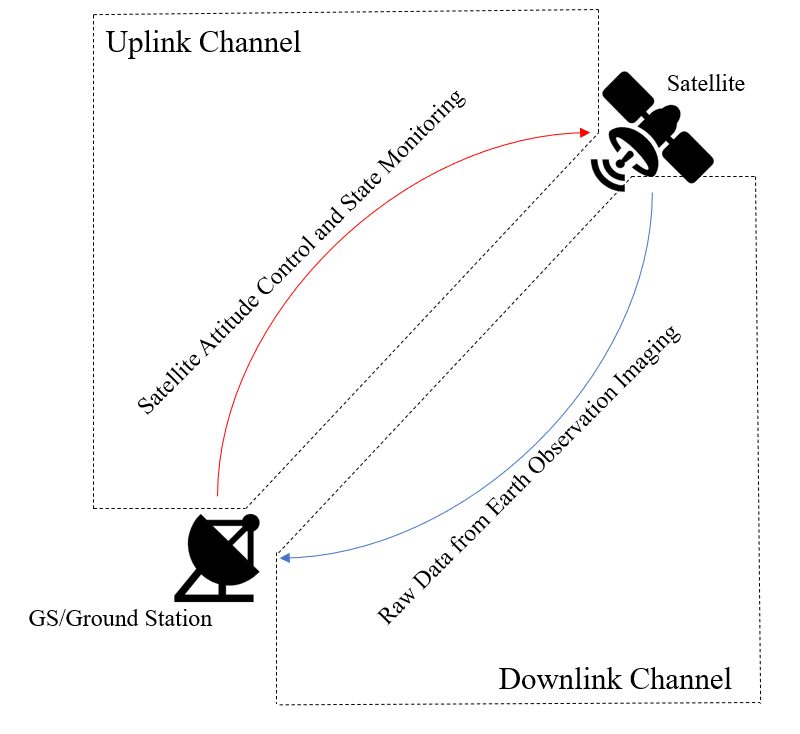
\includegraphics[width=0.5\textwidth]{1.png}
\caption{The traditional manually scheduled satellite computing scheme.}
\label{fig:satellite_ground_model}
\end{figure}

To address this gap, we develop a hybrid model-driven reinforcement-learning framework for sequential scheduling between a satellite and ground infrastructure. The analytical component evaluates the immediate cost of each action using heat generation, floating-point operations (FLOPs), processing and transmission latency, co-location overhead, and bandwidth use. The reinforcement-learning component estimates the long-term value of an action after accounting for its effect on future resource availability. Table~\ref{tab:cost_factors} summarizes the rationale for the immediate cost factors.

\begin{table}
\begin{center}
\caption{Key Cost Factors in Satellite Computational Task Modeling}
\label{tab:cost_factors}
\begin{tabular}{p{2cm} p{4cm}}
\hline
\textbf{Cost Factor} & \textbf{Rationale} \\
\hline
Thermal Output & Strict thermal management is essential in space environments to maintain satellite functionality and prevent system failures. \\
\hline
Computational Load & Limited onboard computing capacity necessitates offloading computationally intensive tasks to ground stations. \\
\hline
Processing Latency & Time-sensitive remote sensing applications require strict adherence to real-time processing constraints. \\
\hline
Co-location Overhead & Concurrent execution of multiple tasks on a single satellite leads to resource contention and reduced efficiency. \\
\hline
Bandwidth Usage & Precious uplink/downlink capacity between satellite and ground requires careful allocation and conservation. \\
\hline
\end{tabular}
\end{center}
\end{table}

Latency constrains time-sensitive applications~\cite{abdulkarim2025multi}, whereas thermal load affects hardware safety in space~\cite{karkadakattil2025ai}. Limited downlink bandwidth can bottleneck data-intensive tasks~\cite{zhang2024dynamic}. Co-located services also compete for shared resources and can reduce overall utility~\cite{10589437}. Finally, onboard computation draws from a finite energy budget~\cite{10589437}. These constraints motivate their joint treatment in the proposed model.


The main contributions of our work are summarized as follows:
\begin{enumerate}
    \item We establish an interpretable immediate-cost model that jointly quantifies thermal load, computation, latency, co-location overhead, and bandwidth use across three processing modes.

    \item We formulate satellite-ground task allocation as a sequential decision process. The state combines task descriptors with evolving thermal, energy, queue, computing, and communication resources, allowing the policy to represent delayed action consequences.

    \item We implement MD-DQN-RSF, which uses model-derived immediate rewards and learns long-term action values. Epsilon reset, selective parameter updates, and replay-buffer flushing are evaluated through cumulative ablation rather than assumed to improve the base learner.

\end{enumerate}



\section{Nomenclature}
\label{sec:symbols}


The subscripts $s$, $g$, and $s\&g$ denote onboard execution, ground-based execution, and satellite-ground collaborative processing, respectively.

\begin{table}[H]
\centering
\caption{Notation Definition}
\label{table:states}
\begin{tabular}{p{2cm}p{1.5cm}p{4cm}}
\hline
\textbf{Scheduling Strategy} & \textbf{\makecell{State \\ Symbol}} & \textbf{State Description} \\
\hline
\multirow{6}{2cm}{Task processed on the satellite} 
& $Q_s$ & Heat cost \\
& $FLOPs_s$ & Computational cost (floating-point operations) \\
& $t^{proc}_{s}$ & Task processing latency \\
& $t^{trans}_{s}$ & Result transmission latency \\
& $f(n)_s$ & Co-location cost (when multiple tasks run simultaneously) \\
& $B_s$ & Bandwidth occupation cost \\
\hline
\multirow{3}{2cm}{Task processed on the ground} 
& $Q_g$ & Heat cost \\
& $t_g$ & Data transmission latency \\
& $B_g$ & Bandwidth occupation cost \\
\hline
\multirow{6}{2cm}{Task preprocessed onboard and further processed on the ground}
& $Q^{pre}_{s\&g}$ & Heat cost during preprocessing \\
& $Q^{trans}_{s\&g}$ & Heat cost during transmission \\
& $t^{pre}_{s\&g}$ & Preprocessing latency \\
& $t^{trans}_{s\&g}$ & Data transmission latency \\
& $FLOPs_{s\&g}$ & Computational cost (floating-point operations) \\
& $B_{s\&g}$ & Bandwidth occupation cost \\
\hline
\end{tabular}
\end{table}

Table~\ref{table:states} lists the task-dependent inputs used by the immediate-cost model. The sequential scheduler additionally uses the dynamic resource variables in Table~\ref{tab:dynamic_states}.

\begin{table}[htbp]
\centering
\caption{Dynamic resource-state variables}
\label{tab:dynamic_states}
\begin{tabular}{p{1.4cm}p{5.3cm}}
\toprule
\textbf{Symbol} & \textbf{Definition} \\
\midrule
$h_t$ & Normalized onboard thermal load at decision step $t$ \\
$e_t$ & Normalized remaining onboard energy \\
$q_t$ & Task-queue occupancy \\
$u_t$ & Onboard computing utilization \\
$b_t$ & Available satellite-ground downlink bandwidth \\
$\tau_t$ & Remaining communication contact-window duration \\
$A_t$ & Workload arriving between decision steps $t$ and $t+1$ \\
$\mu_t$ & Workload completed during the current transition \\
\bottomrule
\end{tabular}
\end{table}

\section{Model-Based Immediate Cost Quantification}
\label{sec:cost_modeling}

This section formulates an analytical model for the immediate operational cost of a scheduling action. It assigns dimensionless coefficients and relative weights to five factors, enabling quantities with different units to be aggregated within a common objective. The model does not determine the final policy by itself. Instead, it supplies an interpretable one-step cost to the reinforcement-learning framework developed in Section~\ref{sec:mdrl}.

\subsection{Cost Factor Modeling}

\subsubsection{Thermal Cost Factor Analysis}

The thermal cost is defined as

\begin{equation}
C_{1} =
\begin{cases}
\rho_{heat} \cdot \omega_{heat} \cdot \tan \!\left( \dfrac{\pi}{2} \cdot \dfrac{Q}{Q_{\text{MAX}}} \right), & Q < Q_{\text{MAX}} \\[10pt]
+\infty, & Q \geq Q_{\text{MAX}}
\end{cases}
\label{eq:heat_cost}
\end{equation}

Here, $C_{1}$ is the thermal component of the total cost. The dimensionless coefficient $\rho_{heat}$ normalizes this component against quantities with different units. The weight $\omega_{heat}$ controls its relative importance. Moreover, $Q$ is task-related heat generation in joules, and $Q_{\text{MAX}}$ is the allowable thermal threshold.

The tangent penalty increases nonlinearly as $Q$ approaches $Q_{\text{MAX}}$ and becomes infinite at the threshold. This form prevents the scheduler from selecting actions that violate the specified thermal constraint.

\subsubsection{Computational Load Cost Factor Analysis}

The computational-load cost is defined as

\begin{equation}
C_{2} = \rho_{comp} \cdot \omega_{comp} \cdot \text{FLOPs}
\label{eq:comp_cost}
\end{equation}

Here, $C_{2}$ denotes computational workload, and $\rho_{comp}$ and $\omega_{comp}$ are its dimensionless coefficient and weight. FLOPs denotes the number of floating-point operations required by a task, measured in mega floating-point operations (MFLOPs).

\subsubsection{Processing Latency Cost Factor Analysis}

The latency component combines processing and transmission delays:

\begin{equation}
C_{3} = \rho_{time} \cdot \left( \omega_{proc} \cdot t^{proc} + \omega_{trans} \cdot t^{trans} \right)
\label{eq:time_cost}
\end{equation}

Here, $C_{3}$ is the latency cost, and $\rho_{time}$ is its dimensionless coefficient. The weights $\omega_{proc}$ and $\omega_{trans}$ correspond to processing and transmission latency. The variables $t^{proc}$ and $t^{trans}$ measure these delays in milliseconds.

\subsubsection{Co-location Overhead Cost Factor Analysis}

The co-location overhead is defined as

\begin{equation}
C_{4} = \rho_{coloc} \cdot \omega_{coloc} \cdot f(n)
\label{eq:colocation_cost}
\end{equation}

Here, $C_{4}$ is the co-location cost, with dimensionless coefficient $\rho_{coloc}$ and weight $\omega_{coloc}$. The function $f(n)$ describes how overhead increases with the number $n$ of tasks executed concurrently onboard.

\subsubsection{Bandwidth Usage Cost Factor Analysis} 

The bandwidth cost is defined as

\begin{equation}
C_{5} =
\begin{cases}
\rho_{bw} \cdot \omega_{bw} \cdot \tan \!\left( \dfrac{\pi}{2} \cdot \dfrac{B}{B_{\text{MAX}}} \right), & B < B_{\text{MAX}} \\[10pt]
+\infty, & B \geq B_{\text{MAX}}
\end{cases}
\label{eq:bandwidth_cost}
\end{equation}

Here, $C_{5}$ is the bandwidth-occupancy cost, with dimensionless coefficient $\rho_{bw}$ and weight $\omega_{bw}$. The variable $B$ is the required downlink bandwidth in megabits per second, and $B_{\text{MAX}}$ is the available downlink capacity.

As with the thermal term, the tangent penalty increases nonlinearly and becomes infinite when $B=B_{\text{MAX}}$. This form discourages actions that approach or exceed the available downlink capacity.

\subsection{Immediate Cost Modeling in the Action Space}

\begin{figure}[htbp]
\centering
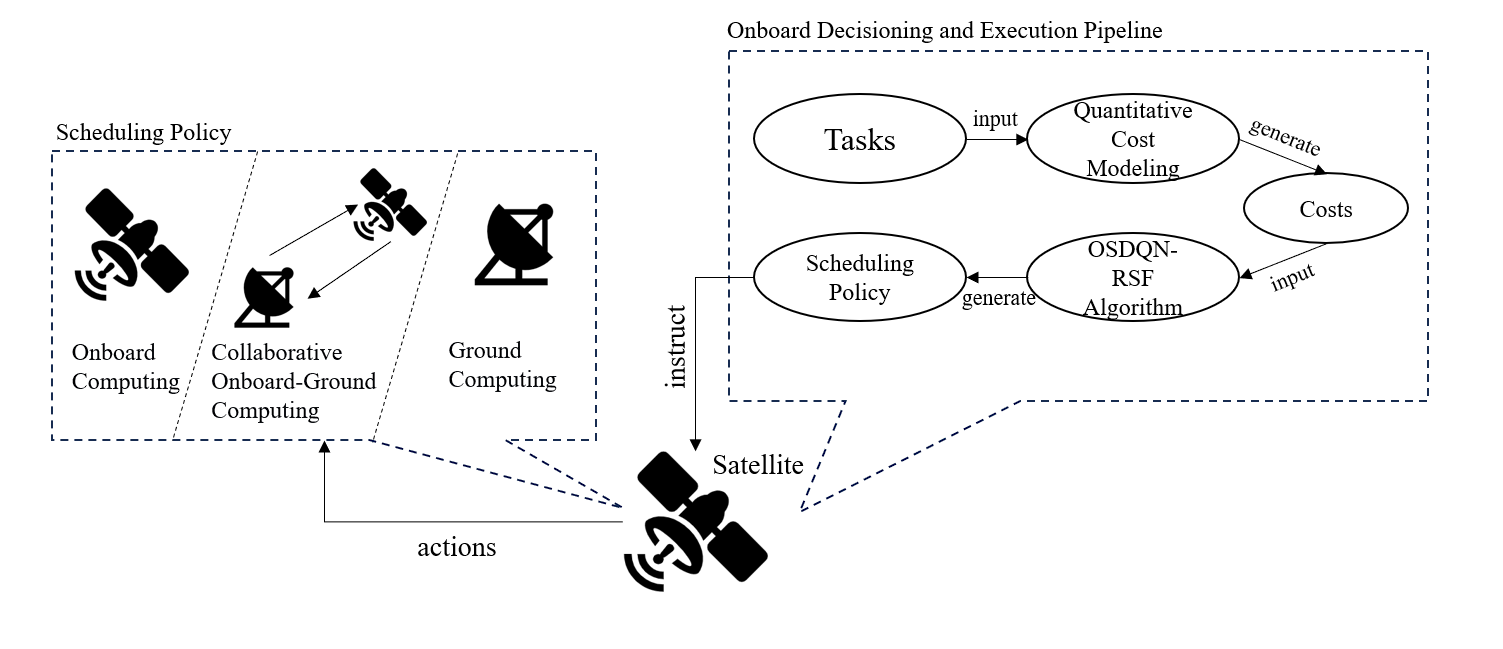
\includegraphics[width=0.5\textwidth]{2.png}
\caption{A schematic diagram of satellite in-orbit decision-making based on model-driven actions within the action space.}
\label{fig:in-orbit decision-making}
\end{figure}

The action space $\mathcal{A}$ contains three processing modes (Fig.~\ref{fig:in-orbit decision-making}):

\begin{equation}
\mathcal{A} = \{\alpha_{s},\alpha_{g}, \alpha_{s\&g}\}
\label{eq:action space}
\end{equation}

\begin{enumerate}
    \item $\alpha_{s}$: the task is processed onboard, and only its result is downlinked.
    \item $\alpha_{g}$: all required data are downlinked and processed on the ground.
    \item $\alpha_{s\&g}$: the data are preprocessed onboard, and the resulting subset is downlinked for further ground-based processing.
\end{enumerate}

The following subsections define an immediate cost for each action. At decision step $t$, the analytical model receives the current task descriptor and resource state, denoted by $x_t$ and $z_t$, respectively. It then evaluates

\begin{equation}
c^{\mathrm{imm}}_t = c_{\mathrm{model}}(x_t,z_t,a_t),
\label{eq:immediate_cost}
\end{equation}

where $a_t\in\mathcal{A}$. The action-specific expressions below define $c_{\mathrm{model}}$. Their input variables are recomputed at each decision step from the current task and available resources. Section~\ref{sec:mdrl} augments this immediate cost with the future consequences of the selected action.

The analytical inputs are therefore conditional estimates rather than fixed task labels. Specifically, the effective transmission latency and bandwidth terms depend on $b_t$ and $\tau_t$, while the co-location term depends on $q_t$ and $u_t$. The action-related heat $Q^{(a_t)}$ and workload determine the increments $\Delta h(x_t,a_t)$ and $\Delta e(x_t,a_t)$ used by the transition model. In the dynamic formulation, $B_{\mathrm{MAX}}$ is replaced by the downlink capacity available at step $t$. This coupling ensures that the same arriving task can have different immediate costs under different resource states.

\subsubsection{Cost Modeling on the Satellite Side}

For onboard execution, the total cost comprises
\begin{itemize}
    \item heat generation cost during task processing,  
    \item computational workload cost measured in floating-point operations,  
    \item task processing time cost on the satellite,  
    \item data transmission delay cost for returning the processed results to the ground,  
    \item co-location cost when multiple tasks are processed simultaneously on the same satellite,  
    \item bandwidth occupancy cost resulting from transmitting the task results to the ground.  
\end{itemize}

The total onboard-execution cost is therefore

\begin{equation}
\begin{aligned}
\mathrm{Cost}_{s} = {} & \; \rho_{\mathrm{heat}}\omega_{\mathrm{heat}}\tan\!\left(\dfrac{\pi}{2}\cdot\dfrac{Q_s}{Q_{\mathrm{MAX}}}\right)
+ \rho_{\mathrm{comp}}\omega_{\mathrm{comp}}\;\mathrm{FLOPs_s} \\
& + \rho_{\mathrm{time}}\left(\omega_{\mathrm{proc}} t^{proc}_{s} + \omega_{\mathrm{trans}} t^{trans}_{s}\right)
+ \rho_{\mathrm{coloc}}\omega_{\mathrm{coloc}}\,f(n)_s \\
& + \rho_{\mathrm{bw}}\omega_{\mathrm{bw}}\tan\!\left(\dfrac{\pi}{2}\cdot\dfrac{B_s}{B_{\mathrm{MAX}}}\right)
\end{aligned}
\label{eq:satellite_cost_sub}
\end{equation}

Here, $\mathrm{Cost}_{s}$ denotes the total cost of onboard execution. The remaining variables are defined in Section~\ref{sec:symbols} and in the preceding cost-factor formulations.

\subsubsection{Ground-Side Cost Modeling}

For ground-based execution, the modeled costs comprise

\begin{itemize}
    \item the thermal cost associated with downlink data transmission from the satellite to the ground,  
    \item the latency cost incurred during transmission, 
    \item the bandwidth occupation cost.  
    \item the computational consumption, heat generation, and latency during computational processes on ground station servers.
\end{itemize}

The ground-based execution cost is therefore

\begin{equation}
\begin{aligned}
\mathrm{Cost}_{g} = {} & \rho_{\mathrm{heat}}\omega_{\mathrm{heat}}
\tan\!\left(\dfrac{\pi}{2}\cdot\dfrac{Q_g}{Q_{\mathrm{MAX}}}\right) \\
& + \rho_{\mathrm{time}}\omega_{\mathrm{trans}}\, t_{g} \\
& + \rho_{\mathrm{bw}}\omega_{\mathrm{bw}}
\tan\!\left(\dfrac{\pi}{2}\cdot\dfrac{B_g}{B_{\mathrm{MAX}}}\right)\\
& + \mathrm{cost}_{ground\_server}
\end{aligned}
\label{eq:ground_cost}
\end{equation}

The term $\mathrm{cost}_{ground\_server}$ represents computation, heat generation, and processing latency at the ground station.

\subsubsection{Satellite-Ground Collaborative Cost Modeling}

For collaborative processing, a task is first preprocessed onboard and then transferred to the ground. The total cost comprises
\begin{itemize}
    \item heat generation cost during onboard preprocessing,  
    \item time cost for preprocessing onboard,  
    \item computational workload cost (FLOPs) for onboard preprocessing,  
    \item transmission delay for sending the preprocessed data to the ground,  
    \item heat generation cost associated with data transmission from the satellite to the ground,  
    \item bandwidth occupancy cost for downlink transmission. 
    \item the computational consumption, heat generation, and latency during computational processes on ground station servers. 
\end{itemize}

The collaborative-processing cost is therefore

\begin{equation}
\begin{aligned}
\mathrm{Cost}_{s\&g} &= \rho_{heat} \omega_{heat}
\tan\!\left(\frac{\pi}{2}\cdot\frac{Q^{pre}_{s\&g}+Q^{trans}_{s\&g}}{Q_{\mathrm{MAX}}}\right) \\
&\quad + \rho_{time} \left( \omega_{pre} t^{pre}_{s\&g} 
+ \omega_{trans} t^{trans}_{s\&g} \right) \\
&\quad + \rho_{\mathrm{comp}}\omega_{\mathrm{comp}}
\mathrm{FLOPs_{s\&g}} \\
&\quad + \rho_{bw} \omega_{bw}
\tan\!\left(\frac{\pi}{2}\cdot\frac{B_{s\&g}}{B_{\mathrm{MAX}}}\right)\\
&\quad + \mathrm{cost}_{ground\_server}
\end{aligned}
\label{eq:sg_cost}
\end{equation}

The term $\mathrm{cost}_{ground\_server}$ has the same definition as in Equation~\eqref{eq:ground_cost}.

Together, these functions permit direct comparison of the immediate costs of onboard, ground-based, and collaborative processing. Selecting the minimum immediate cost provides a transparent myopic baseline, but it does not account for how the selected action changes the costs of subsequent tasks.


\section{Hybrid Model-Driven Reinforcement Learning}
\label{sec:mdrl}

The analytical model in Section~\ref{sec:cost_modeling} evaluates the immediate cost of each processing mode. A scheduler that minimizes this cost independently for every task is myopic because the selected action changes the resources available to subsequent tasks. We therefore formulate scheduling as a Markov decision process and use the analytical model inside the reward. The resulting MD-DQN-RSF framework preserves an interpretable cost decomposition while learning the long-term opportunity cost of each action.

\subsection{Sequential Decision Formulation}

\subsubsection{State Space}

At decision step $t$, the state is

\begin{equation}
s_t = [x_t,z_t],
\label{eq:dynamic_state}
\end{equation}

where $x_t$ contains the task-dependent variables defined in Section~\ref{sec:symbols}. The dynamic resource state is

\begin{equation}
z_t = [h_t,e_t,q_t,u_t,b_t,\tau_t].
\label{eq:resource_state}
\end{equation}

Here, $h_t$ is the normalized onboard thermal load, $e_t$ is the normalized remaining energy, $q_t$ is the task-queue occupancy, and $u_t$ is onboard computing utilization. The variables $b_t$ and $\tau_t$ denote available downlink bandwidth and remaining contact-window duration. This separation distinguishes the properties of the arriving task from resources inherited from previous decisions.

\subsubsection{Action Space}

The action space remains $\mathcal{A}=\{\alpha_s,\alpha_g,\alpha_{s\&g}\}$. These actions correspond to onboard execution, ground-based execution, and onboard preprocessing followed by ground-based processing, respectively.

\subsubsection{State Transition}

Executing $a_t$ changes the resource state before the next task arrives:

\begin{equation}
z_{t+1}=F(z_t,x_t,a_t,\xi_t),
\label{eq:state_transition}
\end{equation}

where $F$ is the satellite-resource transition model and $\xi_t$ represents exogenous task arrivals and link variation. To make the sequential experiments exactly reproducible, all variables are normalized and the implemented transition is

\begin{equation}
\begin{aligned}
h_{t+1} &= \operatorname{clip}\!\left(0.86h_t+0.17c\,\widehat Q_t^{(a_t)},0,1.3\right),\\
e_{t+1} &= \operatorname{clip}\!\left(e_t+0.006-c\,\Delta e_t^{(a_t)},0,1\right),\\
q_{t+1} &= \operatorname{clip}\!\left(q_t+c(\Delta q_t^{(a_t)}-\mu_t^{(a_t)}),0,1.3\right),\\
u_{t+1} &= \operatorname{clip}\!\left(0.68u_t+0.32c\,\widehat w_t^{(a_t)},0,1.2\right),\\
b_{t+1} &= \operatorname{clip}\!\left(\bar b_{t+1}-c\ell_t^{(a_t)},0.08,1\right),\\
\tau_{t+1} &= \operatorname{clip}\!\left(\bar\tau_{t+1}-0.10c\widehat B_t^{(a_t)},0.05,1\right).
\end{aligned}
\label{eq:resource_transition}
\end{equation}

Here, $\widehat Q_t^{(a)}$, $\widehat w_t^{(a)}$, and $\widehat B_t^{(a)}$ are the action-specific heat, workload, and data-demand terms normalized by their sampling maxima. The functions $\Delta e_t^{(a)}$, $\Delta q_t^{(a)}$, $\mu_t^{(a)}$, and $\ell_t^{(a)}$ are deterministic functions of these normalized demands and the current utilization and link state; their implementation is released with the experiment code. The exogenous link variables $\bar b_t$ and $\bar\tau_t$ follow noisy periodic traces generated before an episode begins. The coefficient $c$ controls temporal coupling: $c=0$ removes all action-dependent state transitions and provides the static control, whereas $c=1$ is the nominal sequential setting. Values above one represent stronger-than-nominal coupling.

\subsubsection{Model-Driven Reward}

The analytical model provides the immediate cost $c_t^{\mathrm{imm}}$ in Equation~\eqref{eq:immediate_cost}. To represent operational feasibility, the reward adds continuous hinge penalties for thermal, energy, queue, and contact-window violations:

\begin{equation}
\begin{aligned}
r_t ={}&-c_t^{\mathrm{imm}}-c\big[12(h_{t+1}-0.78)_+
+15(0.18-e_{t+1})_+\\
&\quad+8(q_{t+1}-0.75)_+
+10\,\mathbf{1}_{a_t\ne\alpha_s}(0.14-\tau_t)_+\big],
\end{aligned}
\label{eq:dynamic_reward}
\end{equation}

where $(v)_+=\max(v,0)$. Unlike a direct minimum-cost rule, the action-value function includes future resource consequences:

\begin{equation}
Q^{\pi}(s_t,a_t)=\mathbb{E}_{\pi}\!\left[\sum_{k=0}^{H-t}\gamma^k r_{t+k}\mid s_t,a_t\right].
\label{eq:long_term_value}
\end{equation}

The distinction between $c_t^{\mathrm{imm}}$ and $Q^{\pi}$ is central to the hybrid design. The former remains physically interpretable, whereas the latter represents the expected long-term effect of an action under stochastic task and communication conditions.

\subsection{Model-Driven DQN Architecture and RSF Interventions}
\label{sec:network_architecture}

The action-value network receives the 21-dimensional combined task--resource state and outputs one value for each processing mode. Task inputs are divided by their predefined sampling maxima, and resource inputs are already normalized. The implemented multilayer perceptron has hidden widths of 128, 128, and 64 with rectified-linear activations, followed by three linear outputs. A target network is synchronized every 250 environment steps. Figure~\ref{fig:hybrid_architecture} shows how the analytical immediate-cost model and learned long-term value are combined.

\begin{figure*}[t]
\centering
\includegraphics[width=0.92\textwidth]{md_dqn_rsf/figures/fig_architecture.pdf}
\caption{Hybrid model-driven scheduling architecture. The analytical branch evaluates the interpretable immediate cost of all three processing modes, whereas the value network estimates their cumulative consequences through the dynamic resource state. The selected action updates the satellite--ground system and hence the state presented with the next arriving task.}
\label{fig:hybrid_architecture}
\end{figure*}

MD-DQN-RSF extends the standard DQN~\cite{RN34,RN35,RN36} with epsilon reset, selective parameter updates, and replay-buffer flushing. Their contribution is evaluated individually rather than inferred from the full model alone.

\subsubsection{Motivation for the RSF Mechanisms}

The standard DQN can exhibit inefficient exploration and unstable learning when task arrivals and link conditions produce uneven state coverage. Epsilon reset reintroduces exploration after the network has learned an initial policy. Selective updates limit the influence of high-loss exploratory batches during the reset phase. Replay-buffer flushing subsequently removes older exploratory transitions. These mechanisms are hypotheses rather than assumed improvements; Section~\ref{sec:results} reports their cumulative ablation.

\subsubsection{Epsilon Reset}

The baseline DQN uses an epsilon-greedy policy. Epsilon decays linearly from 1.0 to 0.05 over the first 35\% of the total training steps. In the nominal ablation, the reset variants restore $\epsilon$ to 0.65 at 45\% of the training episodes and decay it to 0.05 a second time. The independent confirmation study calibrates this schedule separately, as described in Section~\ref{sec:rsf_confirmation_protocol}. The reset introduces new exploratory transitions after an initial policy has formed.

\subsubsection{Selective Update}

In the baseline DQN, every scheduled mini-batch produces a backpropagation update. After epsilon reset, MD-DQN-RSF accepts an update only when its Huber loss does not exceed $\kappa$ times the exponential moving average of previously accepted losses. The moving average uses a coefficient of 0.98. The nominal ablation sets $\kappa=1.8$, whereas the confirmation study uses its calibration-locked value. This adaptive rule avoids a scale-dependent fixed loss threshold.

\subsubsection{Flushing Replay Buffer}

The replay buffer stores state, action, reward, next-state, and terminal-indicator tuples. In the nominal ablation, the full method clears the buffer at 72\% of the training episodes and repopulates it under the post-reset policy. Whether this loss of older coverage is offset by faster adaptation is tested empirically in both the nominal and independent ablations.


\begin{algorithm}
\caption{MD-DQN-RSF}
\label{alg:md-dqn-rsf}
\SetAlgoLined

Initialize replay memory $\mathcal{D}$ to capacity $N$\;
Initialize online network $Q_{\theta}$ and target network $Q_{\bar{\theta}}\leftarrow Q_{\theta}$\;

\For{episode $= 1$ \KwTo $M$}{
    Apply the scheduled epsilon reset or replay-buffer flush, if due\;
    Initialize the dynamic environment and observe $s_1=[x_1,z_1]$\;
    
    \For{$t = 1$ \KwTo $T$}{
        With probability $\epsilon$, select a random action $a_t$\;
        Otherwise select $a_t = \arg\max_a Q_{\theta}(s_t,a)$\;
        Evaluate $c_t^{\mathrm{imm}}$ with the analytical model\;
        Execute $a_t$ and observe $r_t$, $s_{t+1}$, and terminal indicator $d_t$\;
        Store transition $(s_t,a_t,r_t,s_{t+1},d_t)$ in $\mathcal{D}$\;
        \If{$t$ is an update step and $|\mathcal{D}|\geq$ batch size}{
            Sample a random mini-batch $(s_j,a_j,r_j,s_{j+1},d_j)$ from $\mathcal{D}$\;
            Set $y_j=r_j+\gamma(1-d_j)\max_{a'}Q_{\bar{\theta}}(s_{j+1},a')$\;
            Compute the Huber loss $L=\mathcal{L}_{\mathrm{Huber}}(y_j,Q_{\theta}(s_j,a_j))$\;
            \If{selective update is inactive OR $L < \kappa\overline L$}{
                Update $\theta$ by one Adam step on $L$\;
            }
        }
    }
    Copy $\theta$ to $\bar{\theta}$ every $C$ environment steps\;
}
\end{algorithm}

Algorithm~\ref{alg:md-dqn-rsf} summarizes the complete procedure. The analytical model enters the algorithm only through the immediate cost and constraint terms. The neural network is therefore not used to approximate a minimum over three known static costs; it estimates how each action changes expected cumulative performance through the transition dynamics.




\section{Experimental Design and Evaluation Protocol}
\label{sec:experiments}

The experiments are designed to test whether learning long-term action values provides an advantage over minimizing the immediate analytical cost. The evaluation therefore separates four questions: whether MD-DQN-RSF improves long-term performance, whether the improvement arises from sequential resource coupling, which RSF mechanisms contribute to learning, and where the learned policy fails.

\subsection{Dynamic Scheduling Scenarios}

Each episode contains 64 arriving remote-sensing tasks. The 15 task variables follow the ranges in Table~\ref{tab:dynamic_ranges}, which preserve the ranges used by the original one-step simulator. All task and exogenous link traces are generated at reset; consequently, policies evaluated with the same seed receive identical arrivals even though their endogenous resource states diverge. Training episode $k$ for model seed $m$ uses seed $10^6m+k$. The 100,000-series seeds were used only for calibration, whereas final testing uses 20 disjoint 500,000-series traces for each model seed.

\begin{table*}[t]
\centering
\caption{Task-variable ranges in each 64-step episode. All continuous variables are sampled uniformly before scenario-specific perturbations.}
\label{tab:dynamic_ranges}
\resizebox{\textwidth}{!}{%
\begin{tabular}{llll}
\toprule
Mode & Heat and computation & Processing/transfer latency & Co-location or bandwidth \\
\midrule
Onboard & $Q_s,\mathrm{FLOPs}_s\in[0,1000]$ & $t_s^{proc}\in[0,1000]$, $t_s^{trans}\in[200,300]$ & $n\in\{0,\ldots,49\}$, $f(n)=n^2$, $B_s\in[0,1000]$ \\
Ground & $Q_g\in[0,1000]$ & $t_g\in[200,20000]$ & $B_g\in[0,1000]$ \\
Collaborative & $Q_{s\&g}^{pre}+Q_{s\&g}^{trans}\in[0,1000]$, $\mathrm{FLOPs}_{s\&g}\in[0,1000]$ & $t_{s\&g}^{pre}\in[0,1000]$, $t_{s\&g}^{trans}\in[200,20000]$ & $B_{s\&g}\in[0,1000]$ \\
\bottomrule
\end{tabular}
}
\end{table*}

For numerical evaluation, the coefficient--weight products in the immediate model are 0.4 for onboard and collaborative tangent heat and bandwidth terms, 0.0004 for FLOPs, 0.0002 for onboard processing and result-transfer latency, and 0.004 for co-location overhead. Ground execution uses $2/3$ for the tangent heat term, 0.0005 for transfer latency, and 0.4 for the tangent bandwidth term. Collaborative preprocessing and transfer latencies both use 0.0004. The effective onboard processing latency is multiplied by $(1+1.4u_t+0.7q_t)$, collaborative preprocessing latency by $(1+0.8u_t)$, co-location overhead by $(1+q_t)$, and ground/collaborative transfer latency by $1/\max(b_t,0.08)$. State surcharges of $0.35h_t+0.12(1-e_t)$ for onboard execution and $0.18h_t+0.12q_t$ for collaborative execution are included. Link-dependent actions also incur hinge surcharges when $\tau_t$ is below 0.28 (ground) or 0.22 (collaborative). Ground-server computation cost is set to zero in this simulator; conclusions therefore concern satellite-side and link resource allocation rather than terrestrial energy optimization.

In the nominal scenario, available bandwidth follows $\bar b_t=0.62+0.23\sin(2\pi t/24+\phi)+\varepsilon_t$, where $\phi$ is uniform on $[0,2\pi)$, $\varepsilon_t\sim\mathcal N(0,0.06^2)$, and the result is clipped to $[0.12,1]$. Contact duration is generated analogously with mean 0.55, amplitude 0.35, period 31, Gaussian noise with standard deviation 0.04, and clipping to $[0.08,1]$. Initial $(h,e,q,u)=(0.22,0.88,0.12,0.18)$. The burst condition multiplies heat- and compute-related demands by 1.45 during one contiguous quarter of the episode. The link-limited condition subtracts 0.22 from available bandwidth before clipping. Energy-limited and thermal-stress episodes begin with $e_0=0.62$ and $h_0=0.42$, respectively; thermal stress also includes the burst perturbation.

\subsection{Comparison Methods}

MD-DQN-RSF is compared under identical task traces and cost parameters with the following policies:

\begin{enumerate}
    \item \textit{Immediate-cost argmin}, which evaluates the three analytical costs and selects the lowest-cost action at each step. This baseline isolates the value of long-term learning from the value of the cost model itself.
    \item \textit{Fixed onboard} and \textit{fixed ground}, which assign every task to one processing location and provide operational reference points.
    \item \textit{Threshold heuristic}, which avoids onboard execution when $h_t>0.72$ or $e_t<0.24$, avoids link-dependent actions when $b_t<0.22$ or $\tau_t<0.14$, selects collaborative execution when $q_t>0.70$, and otherwise uses the immediate argmin.
    \item \textit{Contextual bandit}, which receives the same state variables but optimizes only the immediate reward without temporal bootstrapping.
    \item \textit{Standard DQN}, which uses the same network, state, reward, and training budget without the RSF mechanisms.
    \item \textit{MD-DQN-RSF}, the complete proposed method.
\end{enumerate}

\subsection{Evaluation Metrics}

The primary endpoint is the undiscounted cumulative operational cost per episode. Secondary endpoints are the immediate-cost and penalty components, the numbers of thermal, energy, queue, and contact-window violations, and the fraction of tasks assigned to each processing mode. These metrics distinguish a policy that merely minimizes the current analytical cost from one that preserves resources for future tasks.

\subsection{Statistical Analysis}

Five independently initialized model seeds constitute the experimental units. Within each seed, every policy is evaluated on the same 20 held-out traces; trace metrics are first averaged within the seed and are not treated as independent replicates. Results are summarized as the mean and standard deviation across the five seed-level values. The primary MD-DQN-RSF versus immediate-argmin effect is a paired seed-level mean difference with a two-sided 95\% percentile bootstrap confidence interval from 10,000 resamples (fixed bootstrap seed 20260819). No null-hypothesis significance test or multiplicity-adjusted claim is made for the exploratory secondary comparisons.

Hyperparameters were fixed using the calibration traces before the 500,000-series test traces were generated. Each model was then trained for the prespecified 600 episodes; the terminal model, rather than the best test episode, was evaluated. Experiments used Python 3.13.9, PyTorch 2.8.0+cu129, and one NVIDIA RTX 5070 Ti GPU in the \texttt{yolo} Conda environment. Table~\ref{tab:dynamic_hyperparameters} reports the common training configuration.

\begin{table}[t]
\centering
\caption{Training hyperparameters for the nominal experiment}
\label{tab:dynamic_hyperparameters}
\begin{tabular}{ll}
\toprule
Parameter & Value \\
\midrule
Episodes; steps per episode & 600; 64 \\
Optimizer; learning rate & Adam; $3\times10^{-4}$ \\
Discount factor $\gamma$ & 0.97 \\
Replay capacity; batch size & 100,000; 128 \\
Gradient/target update interval & 4/250 steps \\
Initial/minimum $\epsilon$ & 1.0/0.05 \\
Reset episode; reset $\epsilon$ & 270; 0.65 \\
Flush episode & 432 \\
Selective threshold & $1.8\overline L$ \\
\bottomrule
\end{tabular}
\end{table}

\subsection{Ablation and Sensitivity Analysis}

The cumulative ablation begins with standard model-driven DQN and adds epsilon reset (R), selective updates (R+S), and replay-buffer flushing (R+S+F). Robustness analyses vary temporal coupling from 0 to 1 and evaluate burst, link-limited, energy-limited, and thermal-stress scenarios. A mechanism is considered beneficial only when its improvement is consistent across independent seeds and is not obtained by increasing constraint violations.

\subsection{Independent RSF Confirmation Protocol}
\label{sec:rsf_confirmation_protocol}

We conducted a separate two-stage study to distinguish configuration selection from final RSF assessment. The calibration stage compared six prespecified RSF schedules using four model seeds (100--103) and 20 traces per seed from the 700,000-series namespace. The selection endpoint was the mean seed-level paired total-cost difference between full MD-DQN-RSF and standard MD-DQN. Calibration selected the \texttt{c4\_early\_moderate} schedule, which reset epsilon to 0.50 at 35\% of training, set $\kappa=2.5$, and flushed the replay buffer at 85\% of training.

The selected schedule was locked before the confirmation stage. Standard MD-DQN, DQN-R, DQN-RS, and full MD-DQN-RSF were then trained with ten new model seeds (200--209). Each model was evaluated on 20 disjoint traces per seed from the 900,000-series namespace. Trace values were averaged within each model seed, and all ten seeds were retained as the independent units. Paired mean differences relative to standard MD-DQN used two-sided 95\% percentile bootstrap intervals from 10,000 resamples with fixed seed 20260820. No confirmatory seed was selected, excluded, or replaced according to its observed performance.

\subsection{Evidence Required to Establish Reinforcement-Learning Value}

The central comparison is between MD-DQN-RSF and immediate-cost argmin. Under independent static tasks, both methods are expected to select similar actions, and no reinforcement-learning advantage is claimed. The proposed approach is supported only if it reduces cumulative cost or constraint violations when decisions are temporally coupled. The analysis will therefore report performance as the strength of resource coupling increases from static tasks to burst arrivals, constrained links, and stressed onboard resources.

\section{Results}
\label{sec:results}

\subsection{Long-Term Cost and Constraint Violations}

Table~\ref{tab:main_results} reports the prespecified nominal comparison. MD-DQN-RSF reduced cumulative cost from $395.55\pm16.24$ for immediate-cost argmin to $327.20\pm6.52$, a 17.28\% reduction. The paired seed-level mean difference was $-68.35$ (95\% bootstrap CI, $-77.85$ to $-60.38$). This improvement was not obtained by finding a lower immediate analytical cost: MD-DQN-RSF accepted an 8.80\% higher immediate component ($250.28$ versus $230.05$) but reduced the delayed penalty component by 53.52\% ($76.93$ versus $165.51$).

\begin{table}[t]
\centering
\caption{Nominal test performance. Values are mean $\pm$ SD across five independent model seeds after averaging 20 paired traces within each seed.}
\label{tab:main_results}
\resizebox{\columnwidth}{!}{%
\begin{tabular}{lrrrr}
\toprule
Policy & Total cost & Immediate cost & Penalty & Queue violations \\
\midrule
Immediate argmin & $395.55\pm16.24$ & $230.05\pm3.35$ & $165.51\pm14.17$ & $30.42\pm2.58$ \\
Contextual bandit & $388.97\pm15.17$ & $229.58\pm3.54$ & $159.39\pm13.03$ & $29.60\pm2.66$ \\
Standard MD-DQN & $326.45\pm6.62$ & $250.58\pm5.39$ & $75.88\pm2.64$ & $0.98\pm0.90$ \\
MD-DQN-RSF & $327.20\pm6.52$ & $250.28\pm4.93$ & $76.93\pm3.08$ & $1.60\pm0.84$ \\
\bottomrule
\end{tabular}}
\end{table}

The mechanism is visible in Fig.~\ref{fig:dynamic_results}b. MD-DQN-RSF reduced queue-limit violations from $30.42\pm2.58$ to $1.60\pm0.84$ per episode and energy-limit violations from $38.37\pm0.57$ to $32.07\pm0.90$. Thermal and contact violations were already infrequent. The contextual bandit had nearly the same immediate cost as immediate argmin but retained $29.60\pm2.66$ queue violations, indicating that one-step reward optimization did not capture the delayed queue consequence. Fixed onboard, fixed ground, and threshold policies incurred cumulative costs of $653.03\pm12.27$, $1018.37\pm23.25$, and $708.65\pm21.77$, respectively.

\begin{figure*}[t]
\centering
\includegraphics[width=0.96\textwidth]{md_dqn_rsf/figures_final/fig_results.pdf}
\caption{Sequential scheduling performance. \textbf{a}, Nominal cumulative cost. \textbf{b}, Mean number and composition of nominal constraint violations. \textbf{c}, Evaluation under reduced action-dependent coupling without retraining; the agents were trained at $c=1$. \textbf{d}, Cumulative RSF ablation. Error bars and shaded intervals denote SD across five independent model seeds after 20 traces were averaged within each seed; stacked bars in \textbf{b} show seed-level means.}
\label{fig:dynamic_results}
\end{figure*}

\subsection{When Reinforcement Learning Is Necessary}

The coupling control provides the critical boundary test (Fig.~\ref{fig:dynamic_results}c). When action-dependent transitions and delayed penalties were removed ($c=0$), immediate argmin achieved $177.77\pm2.60$, whereas the policy trained at $c=1$ achieved $211.07\pm6.00$. At $c=0.5$, immediate argmin also remained better ($199.93\pm2.50$ versus $224.61\pm5.19$). The ordering reversed only in the fully coupled nominal setting, where delayed penalties were sufficiently large for value learning to offset its higher immediate cost. Thus, these experiments do not support reinforcement learning for independent per-task optimization; they support it specifically when current actions materially alter later resource feasibility. Because the same $c=1$ agents were transferred to the lower-coupling controls without retraining, the $c=0$ and $c=0.5$ values quantify policy-transfer degradation rather than the best attainable DQN at those coupling levels.

The advantage persisted under all four out-of-distribution stress tests. Relative to immediate argmin, MD-DQN-RSF reduced cumulative cost by 22.22\% under burst arrivals, 15.20\% under limited links, 14.67\% with reduced initial energy, and 22.20\% under thermal stress. Absolute cost remained highest under the link-limited condition ($447.71\pm11.59$), identifying communication scarcity as the most difficult tested regime.

\subsection{RSF Ablation and Learning Dynamics}

In the nominal five-seed ablation, standard MD-DQN achieved $326.45\pm6.62$. Adding reset, selective update, and flushing produced $326.63\pm5.92$, $326.59\pm5.68$, and $327.20\pm6.52$, respectively (Fig.~\ref{fig:dynamic_results}d). The full variant was 0.23\% worse than standard MD-DQN. Figure~\ref{fig:training_curves} further shows that epsilon reset temporarily increased exploratory cost, after which both learners converged to similar levels.

The independent confirmation produced a different mean ordering after calibration-only schedule selection (Table~\ref{tab:rsf_confirmation}). Full MD-DQN-RSF reduced total cost by 1.13 units, or 0.35\%, relative to standard MD-DQN. However, its paired 95\% interval ($-3.09$ to $1.00$) included zero. DQN-RS also had an interval that included zero. Reset alone reduced cost by 1.29 units, or 0.40\%, with a paired interval of $-2.44$ to $-0.25$. Thus, reset showed the most consistent benefit in this study, but adding selective update and flushing did not yield a monotonic incremental improvement.

\begin{table}[t]
\centering
\caption{Independent RSF confirmation after calibration-only configuration selection. Total cost is mean $\pm$ SD across ten model seeds after averaging 20 traces within each seed. Differences are paired against standard MD-DQN; negative values favor the ablation variant.}
\label{tab:rsf_confirmation}
\resizebox{\columnwidth}{!}{%
\begin{tabular}{lrrr}
\toprule
Policy & Total cost & Paired difference & 95\% bootstrap CI \\
\midrule
Standard MD-DQN & $321.65\pm7.22$ & Reference & --- \\
DQN-R & $320.36\pm6.53$ & $-1.29$ & $[-2.44,-0.25]$ \\
DQN-RS & $320.44\pm6.54$ & $-1.21$ & $[-2.92,0.24]$ \\
MD-DQN-RSF & $320.52\pm6.73$ & $-1.13$ & $[-3.09,1.00]$ \\
\bottomrule
\end{tabular}}
\end{table}

Taken together, the two ablations do not establish a stable advantage for the complete RSF package over standard MD-DQN. The defensible contribution remains the hybrid sequential formulation. Among the optional interventions, reset warrants further study, whereas the incremental value of selective update and replay-buffer flushing remains unresolved.

\begin{figure}[t]
\centering
\includegraphics[width=\columnwidth]{md_dqn_rsf/figures_final/fig_training.pdf}
\caption{Training cost for standard MD-DQN and MD-DQN-RSF. Lines show the across-seed mean of the 20-episode rolling cost and shading denotes SD ($n=5$ independent model seeds). Vertical lines mark epsilon reset and replay-buffer flushing.}
\label{fig:training_curves}
\end{figure}

% The superseded one-step experiments remain available in the project history and remote legacy scripts.

\section{Discussion}

The hybrid formulation assigns distinct roles to the analytical model and learned value function. The analytical component provides an interpretable measure of the immediate resource cost of each processing mode, whereas the learned component trades a modest increase in immediate cost for fewer delayed violations. The 53.52\% reduction in the penalty component, despite an 8.80\% increase in immediate cost, is direct evidence of this separation. It also prevents the neural network from being presented as a substitute for evaluating three known static costs.

The need for reinforcement learning is conditional rather than universal. If tasks are independent, all relevant parameters are observed, and an action does not affect later resources, immediate-cost minimization is sufficient. This expectation was borne out at $c=0$, and immediate argmin also remained preferable at $c=0.5$. The learned policy became advantageous only under full coupling and remained advantageous in the four full-coupling stress tests.

The two RSF ablations refine, rather than overturn, this conclusion. The nominal schedule did not improve standard MD-DQN, while the calibration-locked schedule produced a small mean improvement whose interval crossed zero. Reset alone showed the most consistent reduction, but adding selective update and flushing did not improve the mean monotonically. These findings suggest that renewed exploration may help some training regimes, but they do not establish the complete RSF package as uniformly superior.

The present evidence is simulation-based. The task traces are synthetic, the normalized transition coefficients have not been calibrated against spacecraft telemetry, and ground-server computation is outside the objective. The policy can therefore inherit structural error from both the analytical cost model and resource simulator. Moreover, the evaluation contains only one satellite, one ground link, and a discrete three-action space; it does not establish scalability to constellation scheduling or continuous resource allocation. Operational claims require calibration with telemetry or a high-fidelity digital twin, explicit safety constraints rather than reward penalties alone, and validation under orbital and traffic distributions not used here.

\section{Conclusion}

This study develops a hybrid model-driven reinforcement-learning framework for sequential task scheduling in satellite-ground edge computing. The analytical model quantifies immediate onboard, ground-based, and collaborative costs, while the value network estimates delayed resource consequences. In the fully coupled nominal simulator, MD-DQN-RSF reduced cumulative cost by 17.28\% relative to immediate argmin, with a paired 95\% bootstrap interval excluding zero. Most of the gain arose from fewer queue and energy violations. Immediate argmin was better when action-dependent coupling was absent or weakened. Reinforcement learning is therefore justified here by temporal resource coupling, not by the need to approximate a known static minimum. In the independent RSF confirmation, reset alone showed a small consistent benefit, whereas the full package achieved only an uncertain 0.35\% mean improvement over standard MD-DQN. RSF should therefore be treated as an optional training intervention rather than the source of the sequential-learning advantage. These conclusions remain limited to the synthetic task, transition, and communication distributions evaluated in this study.


\bibliographystyle{ieeetr} 
\bibliography{ref}

\makeatletter
% 方法：在 biography 环境开始和结束时插入可调控的垂直间距
\AtBeginEnvironment{IEEEbiography}{\vspace*{-3ex}} % 开始时上移
\AtEndEnvironment{IEEEbiography}{\vspace*{-1ex}}   % 结束时上移，影响下一个传记的间距
\makeatother

\begin{IEEEbiography}[{
\includegraphics[width=1in,height=1.25in,clip,keepaspectratio]{ybc.jpg}}]{Bocheng Yang}
    received the B.E. degree in computer science from Wuhan University, Wuhan, China, in 2025. He is currently pursuing the Ph.D. degree with the School of Aerospace, Harbin Institute of Technology (Shenzhen), Shenzhen, China. His research interests include satellite edge computing and deep reinforcement learning.
\end{IEEEbiography}

\begin{IEEEbiography}[{
\includegraphics[width=1in,height=1.25in,clip,keepaspectratio]{zlj.jpg}}]{Lujie Zheng}
    received the B.Eng. degree in aircraft design and engineering from Dalian University of Technology, Dalian, China, in 2024. He is currently pursuing the M.Eng. degree in aeronautical and astronautical science and technology with the School of Aerospace, Harbin Institute of Technology, Shenzhen, China. His research interests include satellite edge computing and deep reinforcement learning.
\end{IEEEbiography}

\begin{IEEEbiography}[{
\includegraphics[width=1in,height=1.25in,clip,keepaspectratio]{lj.jpg}}]{Jian Liu}
    received the Ph.D. degree from the School of Aerospace, Harbin Institute of Technology (Shenzhen), Shenzhen, China, in 2023. He is currently an Associate Researcher with the School of Aerospace. His research interests include signal processing and nonlinear filtering for urban integrated navigation systems.
\end{IEEEbiography}

\begin{IEEEbiography}[{
\includegraphics[width=1in,height=1.25in,clip,keepaspectratio]{cb.png}}]{Bo Chen}
    (Member, IEEE) received the B.E. degree in aerial photogrammetry and the Ph.D. degree in photogrammetric engineering and remote sensing from PLA Information Engineering University, Zhengzhou, China, in 2002 and 2008, respectively. Since 2020, he has been a Professor with the School of Aerospace, Harbin Institute of Technology (Shenzhen), Shenzhen, China. His research interests include onboard satellite computing, geospatial big data, and spatial information engineering.
\end{IEEEbiography}

\end{document}
